\chapter{Dise\~no}
\epigraph{The effective exploitation of his powers of abstraction must be
regarded as one of the most vital activities of a competent programmer.}%
{Edsger W. Dijkstra}

Al igual que con los requerimientos del software, la descripci\'on detallada del
dise\~no quedo documentada en la ``Especificaci\'on de Dise\~no de Software'' y
que se agrega como anexo. An\'alogamente al capitulo anterior, nos limitaremos
a mencionar solo los aspectos mas relevantes del dise\~no, dejando como lectura
adicional el documento anexo.

\section{Metodolog\'ia}

La metodolog\'ia adoptada para realizar el an\'alisis y descripci\'on del
dise\~no se denomina \ac{RDD}\cite{Wirfs03}. Esta t\'ecnica del dise\~no
orientado a objetos, se enfoca en qu\'e responsabilidades deben ser
cubiertas por el sistema y en cu\'ales ser\'an los objetos responsables de
llevarlas a cabo.

Por ``responsabilidades'' se entiende fundamentalmente lo siguiente:
\begin{itemize}
 \item Las acciones que realiza un objeto.
 \item El conocimiento o la informaci\'on que mantiene un objeto.
 \item Las decisiones que realiza un objeto afectando a otros.
\end{itemize}

\subsubsection{Objetivos del dise\~no}

Como ya mencionamos anteriormente, uno de los requerimientos del software fue
que se respetaran los principios del dise\~no orientado a objetos resumidos en
el acr\'onimo \textbf{SOLID}\cite{Martin00}.
\begin{itemize}
  \item \ac{SRP}
  \item \ac{OCP}
  \item \ac{LSP}
  \item \ac{ISP}
  \item \ac{DIP}
\end{itemize}

En particular se puso especial atenci\'on en respetar los principios \ac{SRP}, 
\ac{OCP} y \ac{DIP} debido a que repercuten directamente en que el sistema sea
mas simple de mantener y extender con nuevas funcionalidades. Adem\'as, el
principio \ac{DIP} es fundamental para lograr un software que sea verificable
mediante la automatizaci\'on de pruebas como se pudo comprobar mas adelante, en
la etapa de ``verificaci\'on''.

\section{Arquitectura}

A continuaci\'on veremos los principales componentes del sistema y siguiendo la
metodolog\'ia adoptada, sus respectivas responsabilidades. En la
Figura~\ref{arquitectura} se puede ver el diagrama UML correspondiente. 

\begin{figure} 
  \centering
  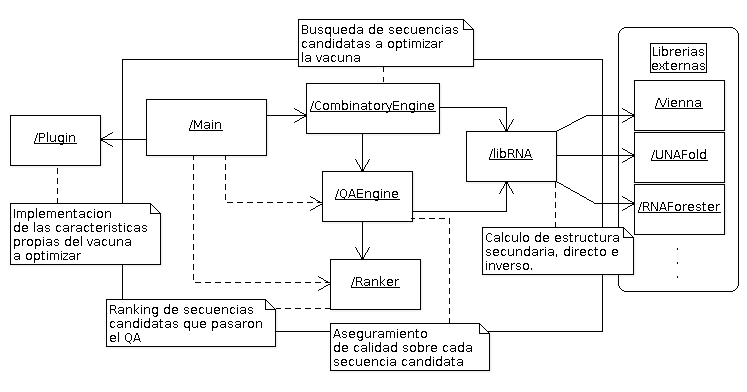
\includegraphics[scale=0.5]{architecture.png}
  \caption{Arquitectura de vac-o.}
\label{arquitectura}
\end{figure}

\begin{itemize}
   \item \textbf{Main:} Representa el componente principal en t\'erminos de
ejecuci\'on del sistema. Comprende principalmente, la inicializaci\'on y
configuraci\'on de otros componentes.
   \item \textbf{Plugin:} Representa la implementaci\'on de las
caracter\'isticas propias de la vacuna que se desea optimizar. Brinda
informaci\'on para la configuraci\'on inicial como as\'i tambi\'en, los
criterios para evaluar las secuencias candidatas.
   \item \textbf{CombinatoryEngine:} Representa el motor combinatorio del
sistema encargado de encontrar, nuevas secuencias que sean candidatas a
optimizar la atenuaci\'on del virus.
   \item \textbf{QAEngine:} Representa el motor de control de calidad del
sistema encargado de decidir, si una secuencia candidata pasa el control o no.
   \item \textbf{Ranker:} Representa el componente encargado de mantener un
``ranking'' de secuencias que sera adem\'as, el resultado final de la
ejecuci\'on.
   \item \textbf{libRNA:} Representa el componente que provee al sistema
funcionalidades para la manipulaci\'on de secuencias y estructuras de \ac{RNA}
(``folding'' directo e inverso y comparaci\'on estructural, entre otras)
utilizando librer\'ias externas.
  \end{itemize}

En las siguientes secciones profundizaremos sobre los componentes ``libRNA'' y
``CombinatoryEngine'' por ser probablemente los mas importantes en cuanto a sus
responsabilidades y dejaremos como lectura adicional la ``Especificaci\'on de
Dise\~no de Software'' que contiene una descripci\'on detallada de todos los
componentes de la arquitectura presentada. Al mismo tiempo, profundizar sobre
estos componentes, nos permitir\'a introducir los principales patrones de
dise\~no que se utilizaron de forma an\'aloga en otras partes del sistema.
Entre otros, se destacan \textit{Iterator}, \textit{Observer}, \textit{Template
Method} y \textit{Visitor}. Para una descripci\'on de estos y otros patrones
del dise\~no orientado a objetos, ver \cite{Gamma95}.

\section{Librer\'ias externas}
\label{diseno-libRNA}
Como vimos en la secciones~\ref{folding} y \ref{inverse}, existen diversas
implementaciones que resuelven el problema de la predicci\'on (directa e
inversa) de estructura secundaria de \ac{RNA} y lo mismo ocurre para el caso de
la comparaci\'on estructural. Adem\'as no se descarta la posibilidad de que en
el futuro aparezcan nuevas y mejores implementaciones. 

Por todo esto, uno de los requerimientos del software fue que sea posible el uso
de cualquiera de estas implementaciones de manera transparente. El problema
radica en que cada librer\'ia tiene diferentes formas de recibir los
par\'ametros de entrada y diferentes formas de dar los resultados que genera. A
ra\'iz de esto se propuso el componente ``libRNA'' como una forma de unificar el
acceso a estas librer\'ias externas e integrarlas al resto del sistema. Las
interfaces propuestas fueron las siguientes:

\begin{itemize}
 \item \textbf{IFold:} Provee la predicci\'on directa (\textit{folding})
de secuencias de \ac{RNA}.
 \item \textbf{IFoldInverse:} Provee la predicci\'on inversa (\textit{inverse
folding}) de secuencias de \ac{RNA}.
 \item \textbf{IStructureCmp:} Provee la comparaci\'on de estructuras
secundarias
de \ac{RNA}.
 \item \textbf{ISequenceCmp:} Provee la comparaci\'on de secuencias de
\ac{RNA}.
\end{itemize}

En esto podemos ver la idea del principio de dise\~no \ac{DIP}. Haciendo que el
sistema dependa de estas interfaces en lugar de sus respectivas
implementaciones conseguimos abstraer los detalles de cada librer\'ia externa y
logramos un software mas vers\'atil. En el capitulo~\ref{librerias} veremos
algunos detalles sobre las implementaciones de estas interfaces y en particular
de \textbf{IFoldInverse}.

\section{Motor combinatorio}

El componente ``CombinatoryEngine'' contiene todo lo referente al recorrido del
espacio de b\'usqueda por lo que es claramente, uno de los componentes
principales de \ac{vac-o}. Esto es fundamentalmente, las regiones
combinatorias y las diferentes estrategias de b\'usqueda.

Para permitir que el software sea de utilidad para diferentes tipos de virus,
tanto las regiones combinatorias como la estrategia de b\'usqueda utilizada
para la optimizaci\'on, deb\'ian ser altamente configurables. Luego, el
objetivo sobre este componente, fue capturar la estructura general de los
algoritmos de b\'usqueda local que suelen denominarse de ``mejoramiento
iterativo''. Algunos de estos algoritmos son:

\begin{itemize}
 \item \textit{First Improvement}
 \item \textit{Best Improvement}
 \item \textit{Simulated Annealing}
 \item \textit{Tabu Search}
\end{itemize}

En todos estos algoritmos, y en general en la b\'usqueda local, est\'an
presentes los conceptos de ``vecindario'' (\textit{neighborhood}) y de
``movimiento'' (\textit{step}) que veremos con mayor detenimiento en el
capitulo~\ref{busqueda}. Mientras tanto, la siguiente introducci\'on nos
servir\'a para justificar las interfaces propuestas.

Si el espacio de b\'usqueda es $\mathcal{S}$, entonces un ``vecindario'' sera
una relaci\'on $\mathcal{N} \subseteq \mathcal{S} \times \mathcal{S}$ y el
``movimiento'' (entre soluciones en el espacio de b\'usqueda) sera una funci\'on
$step: \mathcal{S} \rightarrow \mathcal{D}(\mathcal{S})$. Donde $\mathcal{D}(S)$
denota el conjunto de distribuciones de probabilidad sobre un conjunto dado $S$
y donde una distribuci\'on de probabilidad $D \in \mathcal{D}(S)$ es una
funci\'on $D:S \rightarrow \mathbb{R}^{+}_{0}$ que mapea los elementos de $S$ a
sus respectivas probabilidades.

Luego, en cada iteraci\'on de la b\'usqueda, hay dos responsabilidades bien
diferenciadas e independientes. Por un lado, se debe explorar el ``vecindario''
de la soluci\'on actual. Es decir, si la soluci\'on actual es $s$ y el
``vecindario'' es $\mathcal{N}$, debemos generar el conjunto de soluciones
$\mathcal{N}(s)$. Por otro lado, una vez que se tiene el conjunto
$\mathcal{N}(s)$ de ``vecinos'' de $s$, se debe seleccionar uno de ellos
utilizando la funci\'on $step$. Notar que no siempre la soluci\'on seleccionada
sera mejor que la soluci\'on actual. Inclusive los algoritmos que permiten los
llamados, ``movimientos malos'' (seleccionar con una probabilidad $p$ una
soluci\'on peor que la actual) suelen conducir a mejores resultados.

En este sentido se propusieron la siguientes interfaces:

\begin{itemize}
 \item \textbf{ICombinatoryRegion:} Genera las variantes de la regi\'on
combinatoria que satisfagan la restricci\'on asociada.
 \item \textbf{ISolution:} Representa una soluci\'on en el espacio de
b\'usqueda.
 \item \textbf{INeighborhood:} Explora el vecindario de una soluci\'on.
 \item \textbf{IStrategy:} Decide como pasar de una soluci\'on a la siguiente y
notifica las soluciones que ``mejoran'' a la soluci\'on anterior.
 \item \textbf{ICombinatoryEngine:} Inicia la b\'usqueda y notifica a otros
componentes del sistema las sucesivas soluciones encontradas.
\end{itemize}

Para terminar de entender la interacci\'on entre estas interfaces, en la
Figura~\ref{motor} se puede ver el diagrama de secuencia del motor combinatorio.

\begin{figure} 
  \centering
  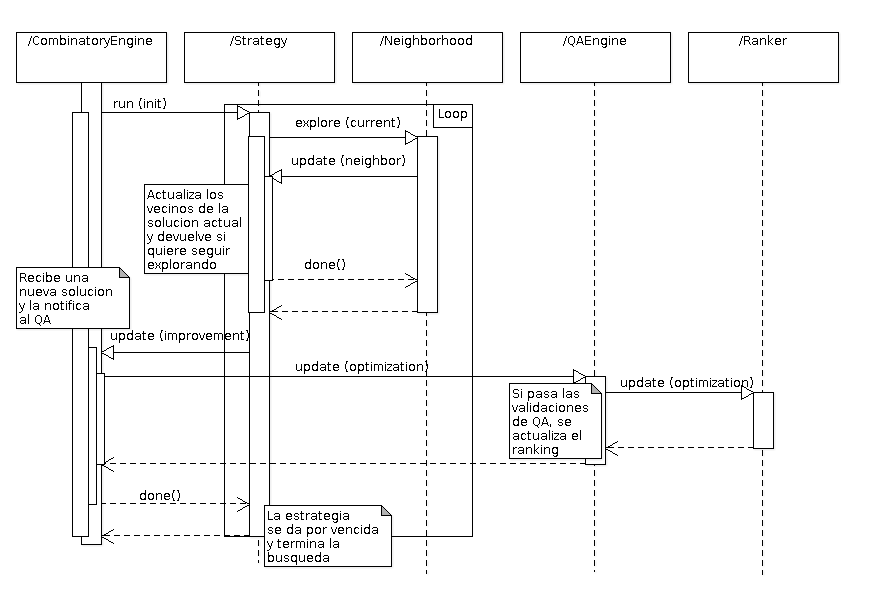
\includegraphics[scale=0.45]{sequence.png}
  \caption{Motor combinatorio de vac-o.}
\label{motor}
\end{figure}

El principal patr\'on de dise\~no que utilizamos en este componente es el que
se denomina \textit{Observer} y que sirve fundamentalmente para lograr la
comunicaci\'on entre diferentes objetos sin que se produzca acoplamiento. La
idea es establecer una relaci\'on entre un emisor y uno, o varios receptores
sin necesidad de generar una dependencia entre el objeto emisor y el objeto
receptor. Adem\'as para permitir el uso del patr\'on \textit{Observer} entre
diferentes tipos de objetos, se propuso el patr\'on de dise\~no \textit{Template
Method}.

En nuestro caso, \textbf{INeighborhood} notifica a \textbf{IStrategy} por cada
soluci\'on que se genera mientras se explora el vecindario de la soluci\'on
actual. Posteriormente, si la soluci\'on seleccionada es mejor que la soluci\'on
actual, \textbf{IStrategy} notifica a \textbf{ICombinatoryEngine} la soluci\'on
seleccionada y este a su vez, la notifica a otros componentes de \ac{vac-o}
(control de calidad).

Una vez mas, remarcamos que las dependencias son entre interfaces y no entre
implementaciones como establece el principio de dise\~no \ac{DIP}. Esto nos
brinda la versatilidad de definir diferentes tipos de regiones combinatorias y
estrategias de b\'usqueda sin modificar en absoluto la implementaci\'on del
motor combinatorio.